\chapter{Experiments}
\label{chap:experiments}
The goal for the experiments is to discover strength and weaknesses for our algorithms and models, given data created by different machines. In section \ref{sec:testenv} the architecture of the used experiment environment is described. In section \ref{sec:pautomac} it is described how Pautomac used 4 parameters for their machines: the state space, the transition sparsity, the emission symbol sparsity and the amount of symbols used in the model. We expect these parameters to produce learning complexity in different ways, where we wish to illustrate how 3 of these 4 parameters effects each algorithm and model, as well as observe an overall logarithmic likelihood score. In an attempt to save time and still produce concise results, we have chosen to use 11 datasets from Pautomac, how these datasets were chosen is described in section \ref{sec:datasets}. In section \ref{sec:parameters} we have studied what parameters the experiments should by run with, including the amount of training data used, \gls{bw}'s threshold and number of \gls{bw} iterations for the \gls{ge} and \gls{gs} algorithm. In section \ref{sec:greedy} we define how many iterations of \gls{bw} that is needed to support strong learning without spending unnecessary amounts of time.
Finally in section \ref{sec:results} the experiments for each parameter experiment can be found. A couple concrete Pautomac competition "submission attempt" has been added as well, to show how our work relates to some of the best results from the competition. In the last section a benchmark of the running time of some algorithms is presented.

\section{Choice of Programming Language}
Initially, Python was used for experimenting with the different algorithms (written in Python) which is provided at the Pautomac website. Python is advantageous in the time it takes to create new or alter existing algorithms, as a dynamically typed and very concise language Python provides for quick writing of new code. However, the Python programming language has been found unsuitable for our needs when continuously running multiple benchmarks to measure the performance of new and existing algorithms due to the long run time.

Several attempts to increase the performance of Python were attempted, such as using different interpreters including the standard Python interpreter, Anaconda and PyPy. Different packages claiming to provide fast calculations of floating points of high precision were also tested. In the end, however, the attempted approaches did not provide satisfactory results leading to a switch to C\# programming language achieving the coveted considerable increase in performance.

Alongside the increase in performance, static types used by  C\# have proved to be very convenient when more people have been working on the same code. Unlike Python, the C\# code has achieved much higher level of readability and adequately served as documentation itself. In many cases, we found that we spent much more time documenting our code when using Python.
\section{Test Environment}

To comply with the need to continuously run multiple extensive experiments and test on both newly proposed algorithms and already existing ``baseline'' algorithms a robust test environment framework has been designed and implemented.

Having the test environment framework common for every tested algorithm made it increasingly simple to set up and evaluate the tests and produce extensive result data as a common interface was implemented for every algorithm to feed it training data and obtain the resulting probabilities.

Another important aspect to the test environment is the ability to reuse existing solutions in multiple algorithms. The experimental algorithms we introduce are mainly based around the well known \gls{baum-welch} and thus the test environment may be utilised to provide unified access to the standard \gls{baum-welch} for every of tested approaches, greatly decreasing the code redundancy and allowing for faster creation and testing of new algorithms in the process.

The test environment thus mainly compromises from several main components. The architecture of the test environment and the dependencies and interoperability of the components are depicted in figure \ref{fig:testenvironment}.

\begin{figure}[!htb]
\centering
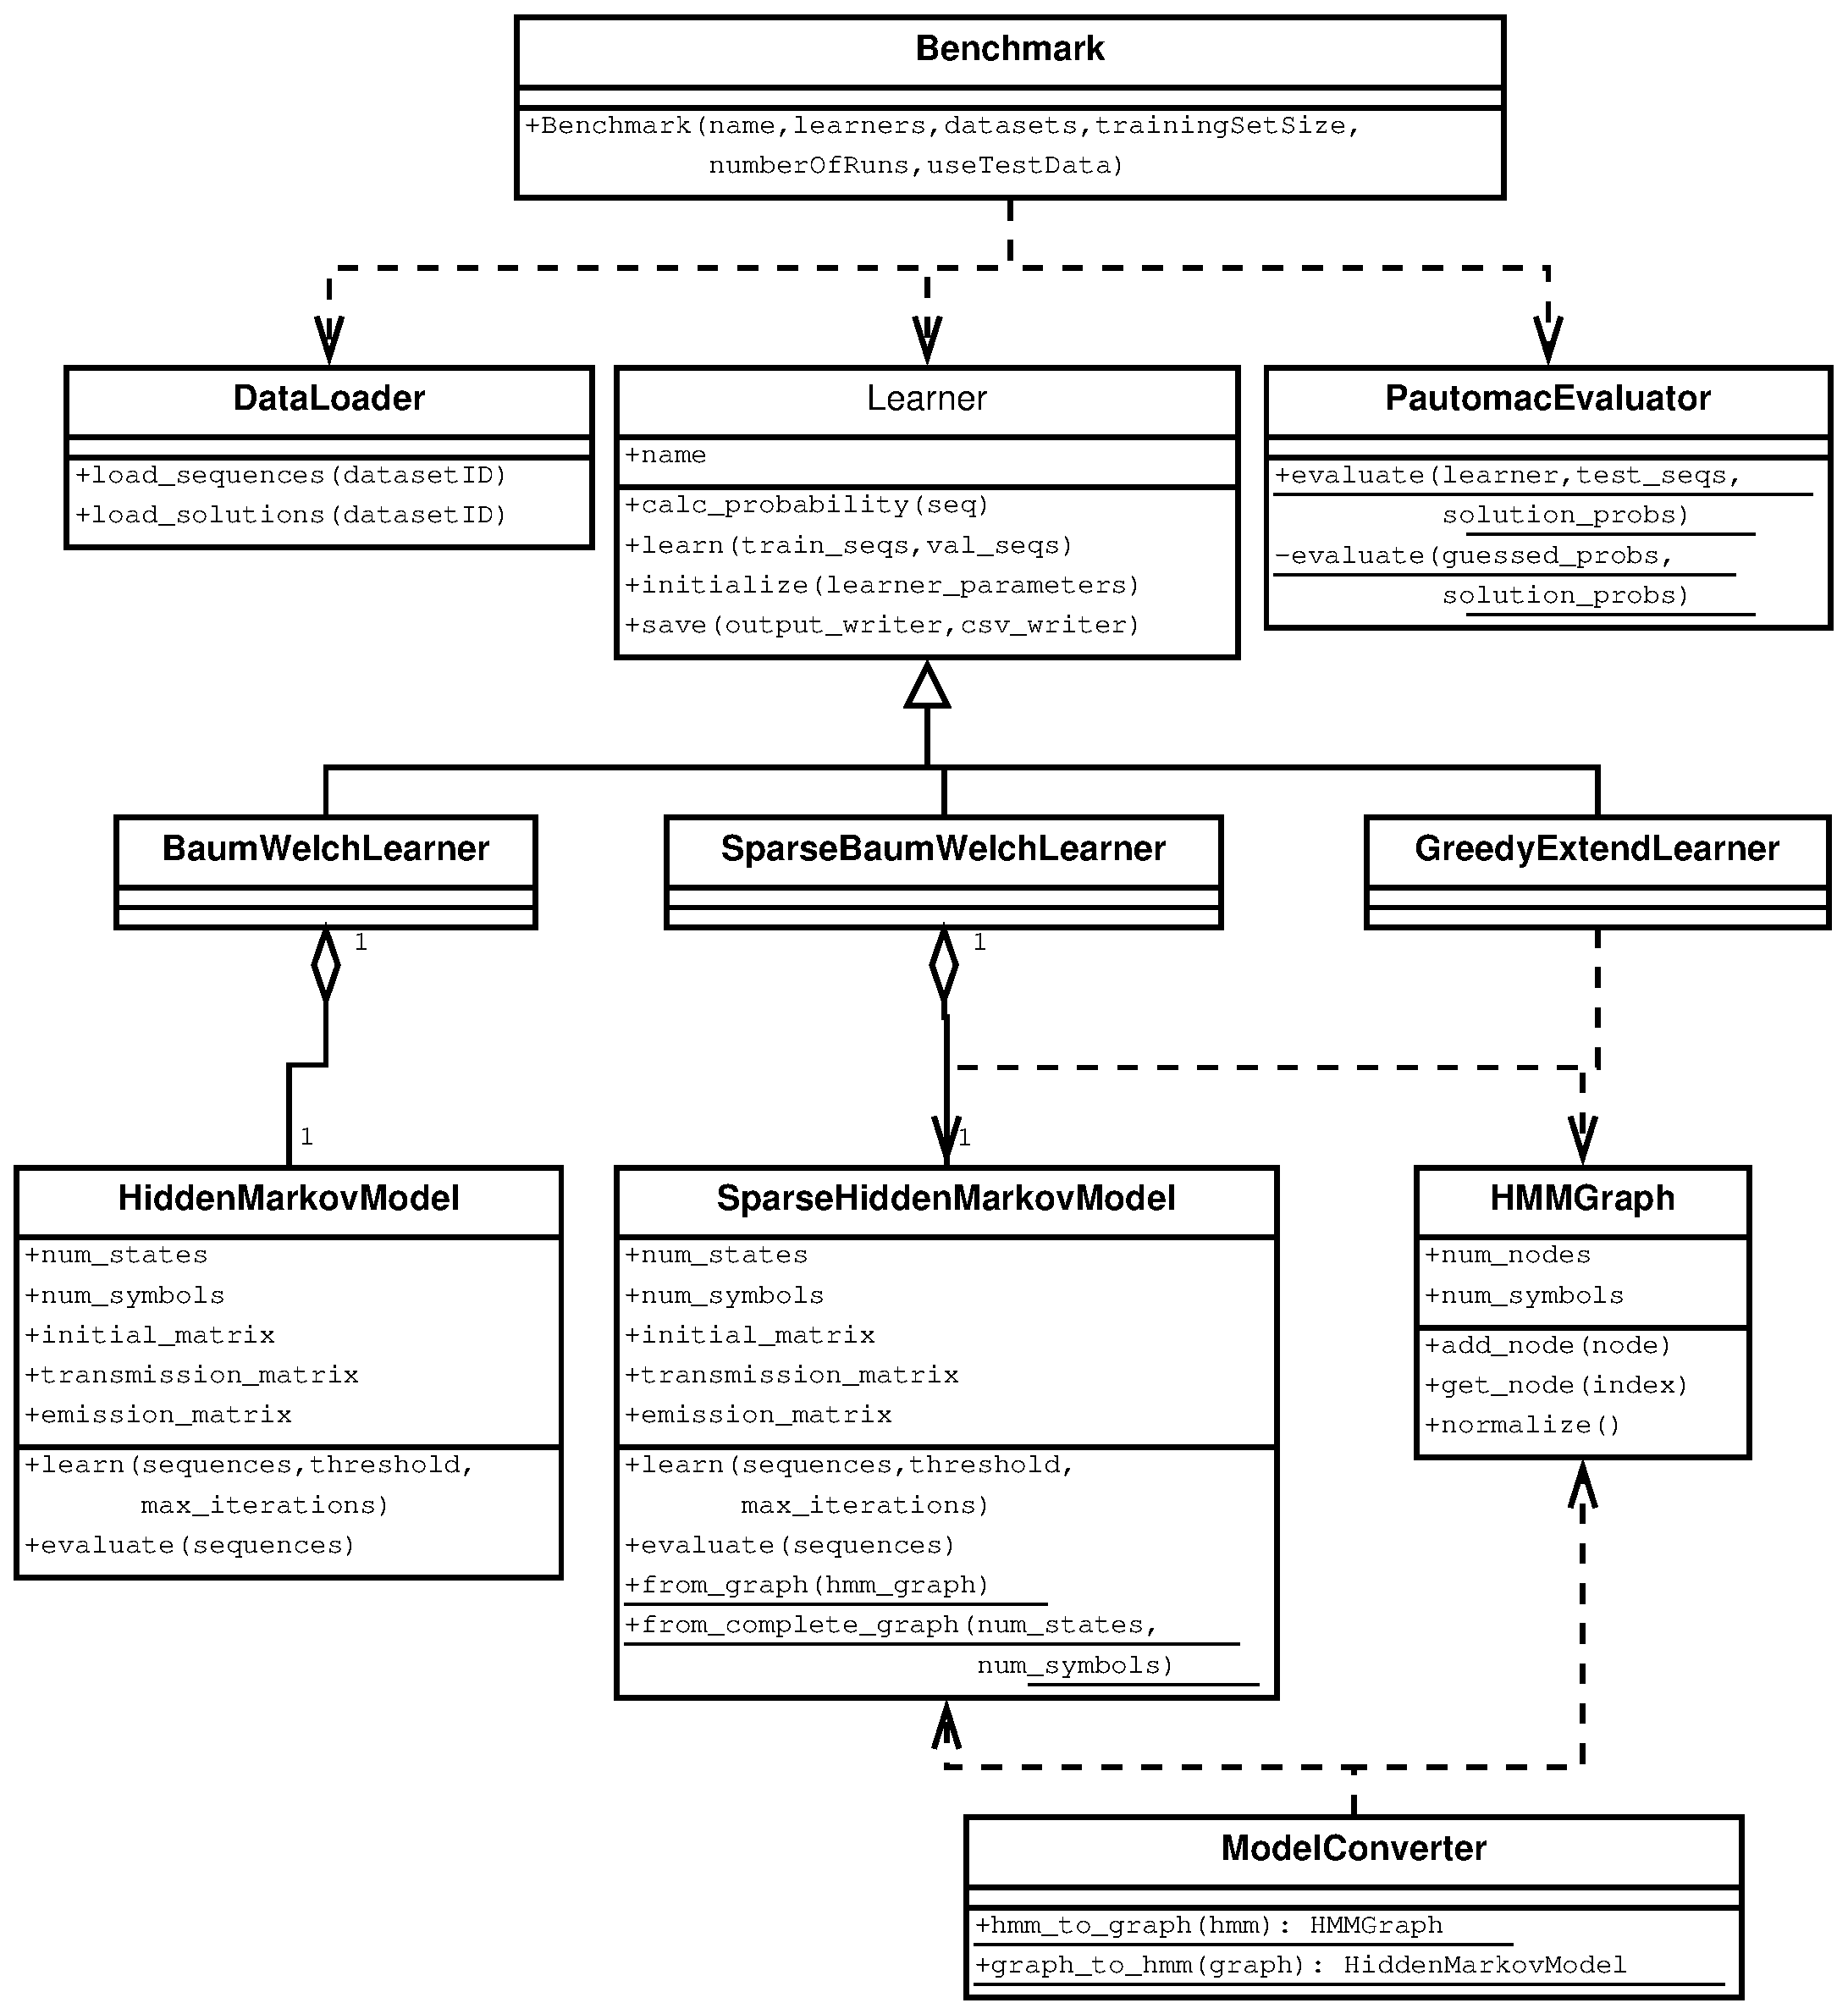
\includegraphics[scale=.4]{pictures/test-environment-overview.eps}
\caption{An overview of the test environment architecture.}
\label{fig:testenvironment}
\end{figure}

\subsection{DataLoader}
The \formatclass{DataLoader} class is responsible for loading both training data, test data and solution data from the files published at the Pautomac website. Both training and test data is represented by a list of sequences, while solution data is represented by a list of probabilities.
This class contains the two functions \formatfunction{load\_probabilities\_from\_file(file\_path)} and \formatfunction{load\_sequences\_from\_file(file\_path)}. The file to be read by both functions must be formatted according to the Pautomac data formats, as described in \todo{insert secref}. The former function outputs a list of sequences, where each sequence is represented by a list of integers.
The latter function outputs a list of probabilities, where each probability is represented by a floating point.

\subsection{Learner}
If one wants to implement a new technique for learning the parameters of a probabilistic model, a new class must be created that derives from the abstract class \formatclass{Learner}.
A learner has only one responsibility: Given a list of training sequences, it must learn a probabilistic model as close as possible to the model used to generate those sequences. How this is done is up to the implementer to choose. The only requirement is that he implements a \formatfunction{calc\_probability(sequence)} function, which given a sequence should return how likely it is that the learned model generated that sequence.
The \formatclass{Learner} class has an already implemented function called \formatfunction{evaluate(sequences, probabilities)}, which uses the \formatfunction{calc\_probability(sequence)} function to calculate probabilities for all provided sequences.
The probabilities are then normalised, and a score is calculated based on the Pautomac evaluation criteria.
The \formatfunction{evaluate} function can be seen by \ref{code:learner}.
A learner should also define a name.

\subsection{Model}
Consider one \formatclass{Learner} that uses the Baum Welch algorithm to estimate the parameters of a Hidden Markov Model and a second \formatclass{Learner} that uses another algorithm, also for estimating the parameters of a Hidden Markov Model. The two learners may need to do many of the same operations on a Hidden Markov Model, e.g. normalization, calculating the probability of being in a particular state or observing a particular sequence at a given time. 
It would be time consuming and increase redundancy if both learners were to implement their own Hidden Markov Model and operations on it.
The \formatclass{Model} has been created to facilitate this. It is an abstract class, which only dictates that a single function must be implemented, which is the \formatfunction{calc\_sequence\_probability(symbol\_sequence)} function. Given a sequence, it must return the probability for the model to generate that sequence. Note that this function is intended to be directly used as the output of the function in the \formatclass{Learner} class having the same name.

\begin{figure}
\caption{The \formatfunction{evaluate} function of the \formatclass{Learner} class.}
\label{code:learner}
\pythonexternal{codeexamples/learner.py}
\end{figure}


\subsection{Evaluator}
This class is responsible for evaluating a \formatclass{Learner} according to the Pautomac evaluation criteria.
Given a learner that has already learned a model, and a number of test sequences with their respective probabilities, it checks how well the probabilities predicted by the \formatclass{Learner} matches the real probabilities.


\subsection{Benchmarker}
For evaluating particular learners on particular data sets, the \formatclass{Benchmarker} class is convenient to use.
As input, it takes a set of learners and data sets, a number of runs, and an output file path.
When run, the \formatclass{Benchmarker} will load all the data sets using the \formatclass{DataLoader}. A data set contains training sequences, test sequences, and a probability associated with each test sequence. For each run, the \formatclass{Benchmarker} randomly splits the training sequences into two sets, where the first $\frac{2}{3}$ sequences are used for training while the remaining are used for validation during training.
Each \formatclass{Learner} will attempt to learn an underlying model for each of the data sets, one by one. When having learned a model for a particular data set, it is evaluated by the \formatclass{Evaluator}. The result of the benchmark is a mean and median score for each pair of learner and data set, which is output to a specified file in .csv format. Besides the mean and median score, the mean and median running time is also measured.
\section{Selecting Datasets}\label{sec:datasets}
In the PautomaC competition, 48 data sets were used. If we were to conduct experiments on all of those data sets, it would take an unreasonable amount of time.
As a consequence, we have chosen to limit the amount of data sets used in our experiments.
We think the most important parameters that differs between data sets are the number of states used by the generating model, the number of symbols, and the transition density. The number of states and symbols have been published after the competition finished, and the transition density is something we can calculate by examining the models that generated each data set, which was also published when the competition finished.
We define the transition density as the ratio between the number of transitions in the model and the number of states squared (the total number of possible transitions). 

For each of the 3 parameters, 4 data sets have been selected that differ as much as possible on that particular parameter, while the other two parameters differ as little as possible.
Figure \ref{fig:statesetplot} shows how four data sets represent different amount of states, while the number of symbols and transition density almost stay the same. In \ref{density_table} and \ref{symbol_table}, a smilar scatterplot can be seen for the transition density and the number of symbols, respectively.

\begin{figure}
	\centering
	\begin{subfigure}[b]{0.5\textwidth}
        	\begin{tikzpicture}
			\begin{axis}[
			scale = 0.8,
			xlabel = Transition density (\%),
            	ylabel = Number of symbols]
			\addplot[scatter,
				only marks,
				scatter src=explicit] 
				table[meta=mark, x=density, y=symbols, col sep=tab]
				{content/Experiments/graphdata/stateset.csv};
			\end{axis}
		\end{tikzpicture}
        \end{subfigure}%
		\begin{subfigure}[b]{0.5\textwidth}
\begin{tikzpicture}
	\begin{axis}[
	scale = 0.8,
			xlabel = Number of states,
            	ylabel = Number of symbols]
		\addplot[scatter,
			only marks,
			scatter src=explicit] 
		table[meta=mark, x=states, y=symbols, col sep=tab]
		{content/Experiments/graphdata/stateset.csv};
	\end{axis}
\end{tikzpicture}
	\end{subfigure}
  	\caption{Two plots visualising the selected state-range datasets}\label{fig:statesetplot}
\end{figure}

%%%%%%%%%%%%%%%%%%%%%%%
%
%_______density range______________

\begin{figure}
	\centering
	\begin{subfigure}[b]{0.5\textwidth}
        	\begin{tikzpicture}
			\begin{axis}[
			scale = 0.8,
			xlabel = Number of states,
            	ylabel = Number of symbols]
			\addplot[scatter,
				only marks,
				scatter src=explicit] 
				table[meta=mark, x=states, y=symbols, col sep=tab]
				{content/Experiments/graphdata/densityset.csv};
			\end{axis}
		\end{tikzpicture}
		\end{subfigure}%
		\begin{subfigure}[b]{0.5\textwidth}
		\begin{tikzpicture}
	\begin{axis}[
			scale = 0.8,
			xlabel = Transition density(\%),
            	ylabel = Number of symbols]
		\addplot[scatter,
			only marks,
			scatter src=explicit] 
		table[meta=mark, x=density, y=symbols, col sep=tab]
		{content/Experiments/graphdata/densityset.csv};
	\end{axis}
\end{tikzpicture}
\end{subfigure}
  	\caption{Two plots visualising the selected density-range datasets}\label{fig:densitysetplot}
\end{figure}

%%%%%%%%%%%%%%%%%%%%%%%
%
%_______symbol range______________

\begin{figure}
	\centering
	\begin{subfigure}[b]{0.5\textwidth}
        	\begin{tikzpicture}
			\begin{axis}[
			scale = 0.8,
			xlabel = Transition density(\%),
            	ylabel = Number of states]
			\addplot[scatter,
				only marks,
				scatter src=explicit] 
				table[meta=mark, x=density, y=states, col sep=tab]
				{content/Experiments/graphdata/symbolset.csv};
			\end{axis}
		\end{tikzpicture}
       \end{subfigure}%
	\begin{subfigure}[b]{0.5\textwidth}
		\begin{tikzpicture}
			\begin{axis}[
			scale = 0.8,
			xlabel = Number of symbols,
            	ylabel = Number of states]
		\addplot[scatter,
			only marks,
			scatter src=explicit] 
		table[meta=mark, x=symbols, y=states, col sep=tab]
		{content/Experiments/graphdata/symbolset.csv};
	\end{axis}
	\end{tikzpicture}
	\end{subfigure}
  	\caption{Two plots visualising the selected symbol-range datasets}\label{fig:symbolsetplot}
\end{figure}

\FloatBarrier

\begin{table}
\centering
{
\begin{tabular}{| c | c | c | c |}
  \hline
  Dataset 	& \textbf{States} 	& Density (\%) 	& Symbols \\  \hline
  6 			& \textbf{19 }			&	13.5				& 6 \\
  23 			& \textbf{33} 			&	11.4				& 7 \\
  41			& \textbf{54} 			&	14.3				& 7 \\
  1				& \textbf{64} 			&	8.7				& 8 \\ \hline
\end{tabular}
\caption{State amount}
\label{state_table}
}
\end{table}

\begin{table}
\centering
{
\begin{tabular}{| c | c | c | c |}
  \hline
  Dataset 	& States  			& \textbf{Density (\%)} 		& Symbols \\  \hline
  36 			&	54					& \textbf{7.4 }						& 9 \\
  8 			&	49					& \textbf{16.8 }					& 8 \\
  43			&	67					& \textbf{40.2 }					& 5 \\
  37			&	69					& \textbf{54 	}					& 8 \\ \hline
\end{tabular}
\caption{Transition density percentage}
\label{density_table}
}
\end{table}

\begin{table}
\centering
{
\begin{tabular}{| c | c | c | c |}
  \hline
  Dataset 	& States	 	& Density (\%) 	& \textbf{Symbols}	 \\  \hline
  32 			& 43				& 11.8				& \textbf{4}		\\
  8 			& 49				& 16.8 				& \textbf{8}		\\
  10			& 49				& 14.2 				& \textbf{11}	\\
  35			& 47				& 14.2 				& \textbf{20}	\\ \hline
\end{tabular}
\caption{Symbol alphabet size}
\label{symbol_table}

}
\end{table}
\subsection{Experiment Parameters}\label{sec:parameters}

Since the static learners use a \gls{hmm} internally, the number of states used may affect the outcome of the experiments.
The Pautomac models that generated the data sets were generated by at most 73 states, and due to the fact, that the computation effort increases quadratically with the number of states, we deem it unnecessary to test models with more than 100 states. Due to the large amount of time it takes to run the \gls{baum-welch}, a step size of 10 for the number of states tested.
The dynamic learners does not require a specified number of states, as they all start with a model containing just a single state, which in turns are extended.

The data sets given by Pautomac ranges in sequences. Some have 20.000 sequences while others have 100.000. These amounts of sequences are however larger than what is necessary to illustrate how one algorithm behaves, given some dataset. Another problem is that the larger datasets takes significantly longer to compute, compared to a subset of sequences. It is therefore interesting to explore what amount of sequences that will both produces useful results, without spending an unnecessary amount of time doing the computations.

\paragraph{Training Sequences}
The Pautomac training sets contain between 20,000 and 100,000 sequences.
An experiment has been conducted, to see whether all of these sequences are needed to learn a good model using \gls{baum-welch}.
The result is depicted in Figure \ref{fig:sequences}. It seems like it does not improve the result significantly when using more than 100 sequences.
However, it was decided to use 5000 sequences as the running time of \gls{baum-welch} for this amount is still reasonable. It should be noted that the running time increases linearly with the amount of sequences used for training, but quadratically by the number of states, following the complexity of the \gls{fb_algorithm} algorithm.

The setup for this experiment:
\begin{itemize}
\item Dataset: 36
\item Algorithm: Baum Welch
\item Threshold: 0.01
\item Training sequences: 100-50,000
\item Validation sequences: 1,000
\item CPU: 2 Ghz Intel core 2 duo
\end{itemize}

\begin{figure}
	\centering
	\begin{subfigure}[b]{0.5\textwidth}
        \begin{tikzpicture}
		\begin{axis}[
				scale = 0.9,
				ymin = 23000,
				ymax = 24000,
				ybar,
				xtick=data,
   				symbolic x coords={100,500,1000,5000,10000,50000},
				xlabel = Sequences,
            		ylabel = Score (lower is better)]
				\addplot+table[y=score, col sep=tab]
				{content/Experiments/graphdata/sequences.csv};
		\end{axis}%
	\end{tikzpicture}
        \end{subfigure}%
		\begin{subfigure}[b]{0.5\textwidth}
\begin{tikzpicture}
		\begin{axis}[
				scale = 0.9,
				ymin = 0,
				ybar,
				xtick=data,
   				symbolic x coords={100,500,1000,5000,10000,50000},
				xlabel = Sequences,
            		ylabel = Running time (seconds)]
				\addplot+table[y=time, col sep=tab]
				{content/Experiments/graphdata/sequences.csv};
		\end{axis}%
	\end{tikzpicture}
	\end{subfigure}
  	\caption{Plot of Baum-welch score and runningtime on different sequence amounts}\label{fig:sequences}
\end{figure}


\paragraph{Baum-Welch Treshold}
The Baum-Welch algorithm takes two parameters, the amount of states which the trained model should consist of and the threshold of convergence. The state range for the experiments have already been selected to range between 10 and 100 with a step size of 10. Unlike the choice of states, which is a variable, the threshold should be a static value for all the experiments.

Defining the threshold is done by exploring how Baum-Welch behaves on different threshold values. \ref{fig:threshold} shows the results from the experiments. Each threshold parameter value were combined with the parameter of 50 states, and trained on a single dataset.

\begin{figure}
\centering
	\begin{tikzpicture}
		\begin{axis}[
				ybar,
				xtick=data,
   				symbolic x coords={0.1,0.05,0.01,0.005,0.001,0.0001},
				xlabel = Treshold,
            		ylabel = Score (lower is better)]
				\addplot+table[y=Score, col sep=tab]
				{content/Experiments/graphdata/treshold.csv};
		\end{axis}
	\end{tikzpicture}
\caption{Negative logarithmic likelihood when running Baum-Welch with different thresholds.}
\label{fig:threshold}
\end{figure}

Based on the results, it is clear that a threshold of 0.01 will produce useful that are representative for much lower thresholds.

\subsection{Greedy Extend}
10 BW iterations between when after each extend.
100 attempts to extend graph.
0.01 threshold for BW when reaching a maximum of 100 states or if not able to expand further.

Whether we choose to run Greedy Extend a single or multiple times does not seem to have a big impact on the result.
In figure \ref{fig:ge-diversity-5-runs}, the result of 5 different runs of Greedy Extend can be seen. The results of all runs look very similar.
\begin{figure}
\begin{centering}
\begin{tikzpicture}
	\pgfplotsset{every axis legend/.append style={ 
		at={(0.5,1.03)},
		anchor=south}}
	\begin{axis}[
			xlabel = Number of states,
            	ylabel = Score (lower is better),
            	legend columns=-1,
            	legend entries={Run 1, Run 2, Run 3, Run 4, Run 5},
			legend style={/tikz/every even column/.append style={column sep=0.3cm}}]
		
		\addplot+[mark=none]table[x=States, y=Run1, col sep=tab]
		{content/Experiments/graphdata/ge-diversity-5-runs.csv};
		
		\addplot+[mark=none]table[x=States, y=Run2, col sep=tab]
		{content/Experiments/graphdata/ge-diversity-5-runs.csv};
		
		\addplot+[mark=none]table[x=States, y=Run3, col sep=tab]
		{content/Experiments/graphdata/ge-diversity-5-runs.csv};
		
		\addplot+[mark=none]table[x=States, y=Run4, col sep=tab]
		{content/Experiments/graphdata/ge-diversity-5-runs.csv};

		\addplot+[mark=none]table[x=States, y=Run5, col sep=tab]
		{content/Experiments/graphdata/ge-diversity-5-runs.csv};
	\end{axis}
\end{tikzpicture} 
\caption{5 different runs of Greedy Extend on the same data set using $\alpha = 100, \beta = 10$.}
\label{fig:ge-diversity-5-runs} 
\end{centering}
\end{figure}

\subsection{Dataset Parameter Experiment}
\label{sec:dataset_experiments}
The approach used for each dataset parameter experiment have been to cover a range of state amounts, ranging from 10 to 100 states alongside the previously defined parameters. \gls{bw} and \gls{sbw} were probed on specific state amounts with step sizes of 10, where the dynamic algorithms have been defined to reach either some local maxima or stop at 100 states.
\subsection{Speed Comparison}

Apart from scoring the individual learning algorithms by logarithmic likelihood or PautomaC evaluation criterion we have also recorded their running time. A special test was conducted to determine the performance benefits of sparsity and other approaches. The Baum-Welch Learner and Sparse Baum-Welch Learner were run for a model of size $5$ and subsequently on models $5$ hidden state larger. Both algorithms were run for exactly 8 hours to observe what results can be obtained during the given time frame. The Greedy Extend Learner was also run for 8 hours to see if the achieved growth can be faster than continuous tests on aforementioned algorithms.

The experiments were conducted using PautomaC dataset number 23. This dataset was chosen as the underlying model used by PautomaC had an average amount of states (33), rather low transition density (11.48\%) and number of symbols (7) making it considerably simple, but not too much. The experiments were run with the same parameters as the main tests, thus with convergence threshold of $0.01$, and a training and validation sets of $5000$ sequences.

The obtained results as shown in regard to score (graph \ref{fig:eight_hour_run}) and running time(graph \ref{fig:bw_vs_sbw}) are speaking in favour of the Greedy Extend Learner, whilst Sparse Baum-Welch Learner achieved the worst performance. This might be attributed to the fact that the transition matrix for the Sparse Baum-Welch Learner is randomly generated, thus even the $nlog(n)$ non-zero transitions are picked by random and the topology of the hidden state space graph cannot be considered data derived.

The tests were run on the same machine as the average speedup tests for the \hyperref[sec:shmm]{Sparse hidden Markov model} with the following configuration:
\begin{itemize}
	\item[] Intel Core i7-4700MQ processor clocked at 2.4 GHz.
	\item[] 8 GB \gls{ram}.
	\item[] Microsoft Windows 8 operating system.
\end{itemize}

\begin{figure}
	\centering
	\begin{tikzpicture}
		\begin{axis}[
			width=0.92\textwidth,
			height=0.76\textheight,
			ymin=0,
			xmin=0,
			xlabel = Number of States,
            		ylabel = Negative Logarithmic Likelihood,
            		legend style={at={(0,0)}, anchor=south west}]
			\addplot+[mark=none]table[x=States, y=Score, col sep=tab]
			{content/Experiments/graphdata/8h_run_BW.csv};
			\addlegendentry{Baum-Welch Learner}
			\addplot+[mark=none]table[x=States, y=Score, col sep=tab]
			{content/Experiments/graphdata/8h_run_SBW.csv};
			\addlegendentry{Sparse Baum-Welch Learner}
			\addplot+[mark=none]table[x=States, y=Score, col sep=tab]
			{content/Experiments/graphdata/8h_run_GE.csv};
			\addlegendentry{Greedy Extend Learner}
		\end{axis}
	\end{tikzpicture}
	\caption{Results achieved in a time scope of eight hours.}
	\label{fig:eight_hour_run}
\end{figure}

In regards to logarithmic likelihood we may observe from the result graph \ref{fig:eight_hour_run} that both Baum-Welch and Sparse Baum-Welch Learners reach what could be called a convergence of the logarithmic likelihood score when increasing the number of states. The relatively stable value is reached at around 45 states for the Baum-Welch Learner with all the subsequent logarithmic likelihoods ranging from $50057.19$ (130 states) to $49718.1$ (80 states). The convergence is a little slower for the Sparse Baum-Welch Learner starting at around 55 states and ranging from $51856.74$ (75 states) to $50736.94$ (180 states).

Unlike the Baum-Welch and Sparse Baum-Welch Learners, the Greedy Extend Learner did not reach convergence during the 8 hours of continuous run. On the other hand the logarithmic likelihood of the Greedy Extend Learner continued to improve as more states were included into the model with an increasing rate of improvement nonetheless. During the 8 hours the Greedy Extend Learner was capable of achieving logarithmic likelihood of $17147.35$ with 352 states.

The difference between the continuous improvement of Greedy Extend and the stable value reached by Baum-Welch and Sparse Baum-Welch Learners can be attributed to the difference in the increase in the number of states. Whilst Baum-Welch and Sparse Baum-Welch Learners increase simply by creating a whole new model with more states that has to be re-learned from the very beginning, the Greedy Extend adds states one-by-one keeping the original model intact. Thus one may argue that the Greedy Extend Learner uses a property very alike to simulated annealing were it attempts to find the global maximum in a smaller and simpler -- less dimensional space of the smaller model first, were the number of local maxima is limited. Once such a maximum is found, the model stays in close proximity to the maximum after the model expands into far more dimensions and the learning continues.

Another possible explanation may be the number of iterations. It has been observed throughout the runs that Baum-Welch and Sparse Baum-Welch Learners showed a declining number of iterations until convergence with increase in the number of states (less than 100 iterations for models around 150 states against as much as 500 iterations for models 20 states and smaller for the Baum-Welch Learner). The Greedy Extend however runs a fixed number of \gls{baum-welch} iterations (tested with $\beta = 10$) each time a new state is added.

The decreasing number of iterations with increasing number of states observed (mostly for Baum-Welch Learner) is suggesting a lower convergence threshold may be required for larger models. More tests with different thresholds are however necessary to confirm this hypothesis.

\begin{figure}
	\centering
	\begin{tikzpicture}
		\begin{axis}[
			width=0.92\textwidth,
			height=0.32\textheight,
			ymin=0,
			xmin=0,
			xlabel = Number of States,
            		ylabel = Time until Convergence {[s]},
            		legend style={at={(0,1)}, anchor=north west}]
			\addplot+table[x=States, y=Time, col sep=tab]
			{content/Experiments/graphdata/8h_run_BW.csv};
			\addlegendentry{Baum-Welch Learner}
			\addplot+table[x=States, y=Time, col sep=tab]
			{content/Experiments/graphdata/8h_run_SBW.csv};
			\addlegendentry{Sparse Baum-Welch Learner}
		\end{axis}
	\end{tikzpicture}
	
	
%	\begin{tabular}{| c | c | c | c | c | c | c | c | c | c | c |}
%		\hline
%		\# of States & 5 & 25 & 50 & 75 & 100 & 120 & 140 & 160 & 180 & 200 \\ \hline
%		Baum-Welch & 22 s & 4.5 m & 6.5 m & 9.5 m & 13 m & 19.5 m & 28 m & 34.5 m & -- & -- \\ \hline
%		Sparse B-W & 25 s & 4 m & 7 m & 15 m & 19 m & 17 m & 15 m & 13 m & 20 m & 18 m \\ \hline
%	\end{tabular}
	\caption{Running time comparison between Baum-Welch and Sparse Baum-Welch Learners.}
	\label{fig:bw_vs_sbw}
\end{figure}

Interesting results are offered by the graph \ref{fig:bw_vs_sbw} comparing the running times of Baum-Welch and Sparse Baum-Welch Learners. One can immediately notice large instability in the running times of the Sparse Baum-Welch Learner. Contrary to the expectations the longest runtime (28 minutes and 47 seconds) was measured for 80 state model whilst the 200 hundred state model only required 11 and a half minutes, even less than the 60 state model with 15 minutes and 8 seconds. This unpredictable behaviour can be attributed mostly to the heavy randomness of the models used by the Sparse Baum-Welch Learner. With the topology of the sparse hidden state graph being random it is likely that a suitable topology is generated for some models whilst a highly unsuitable may be generated for different models leading to increased number of iterations until convergence.

Significantly less unstable behaviour was measured for the Baum-Welch Learner. One can still notice models for which the running time is unusually high (55 states with 16 minutes and 4 seconds) or low (40 states with 3 minutes and 36 seconds) compared to the expectation derived from the trend of the line. This can once again be attributed to the random generation of the initial models. One can see however that with the complete graph topology \gls{baum-welch} is generally able to converge in similar number of iterations as with different random initial parameters.

The longest run measured for the Baum-Welch Learner was for the highest achieved number of states, 160 with 34 minutes and 34 seconds. The achieved running times for the Baum-Welch Learner are generally smaller than expected, mostly for the larger models. This is attributed mostly to the declining number of iterations required until convergence with the growing size of the model. Nevertheless a generally longer running time is measured for the Baum-Welch Learner than the Sparse Baum-Welch Learner with models beyond 100 states large. The graph \ref{fig:bw_vs_sbw} also suggests the gap to continue to widen with more states.

The high diversity in the running time of the Sparse Baum-Welch Learner has inspired us to explore whether more iterations (and therefore longer runtime) are correlated to better (thus smaller) score. We have computed \gls{cor_coefficient} between the logarithmic likelihood and running time for both the Baum-Welch and Sparse Baum-Welch Learners. In both cases the score and the computation time appear to be positively correlated ($r_{BW} = 0.4279$ for Baum-Welch and $r_{SBW} = 0.6328$ for Sparse Baum-Welch). This is mostly attributed to the sharp increase in both running time and logarithmic likelihood (observable as decrease in negative logarithmic likelihood in graph \ref{fig:eight_hour_run}) measured for small models, before the stable value was reached. Much more interesting might therefore be to measure the correlation only for the models that are already scoring close to the stable value (45 states and beyond for Baum-Welch and 55 states and beyond for Sparse Baum-Welch).

The \gls{cor_coefficient} between logarithmic likelihood and running time for the Baum-Welch Learner on models at least 45 states large shows a slight negative correlation ($\overline{r_{BW}} = -0.1134$). This can be attributed to continued increase in running times but only meek changes in the logarithmic likelihood nonlinear in regard to number of states.

On the other hand the \gls{cor_coefficient} for the Sparse Baum-Welch Learner shows considerably high positive correlation ($\overline{r_{SBW}}=0.5035$). This shows that the highly unstable running times have non-negligible impact on the score the algorithm achieves. \gls{cor_coefficient} does not climb close to 1, however, thus we may assume that the number of iteration taken and in turn the running time of the algorithm does not directly translate to the improvement of the score. This may again be attributed to the random topology of hidden state space graphs.

It should be noted that the experiments in this section were conducted solely on one dataset. It might be necessary to confirm the derived results by running the tests on different data. This is also supported by the fact that vastly different running times were measured for individual datasets when performing other test sets.
